\section{$A_5[1^-2^-3^+4^+5^+]^{\mathrm{1-loop}}$ in N=4}
There are four possible configurations contributing to the quadruple cut.
\begin{figure}[h!]
  \centering
    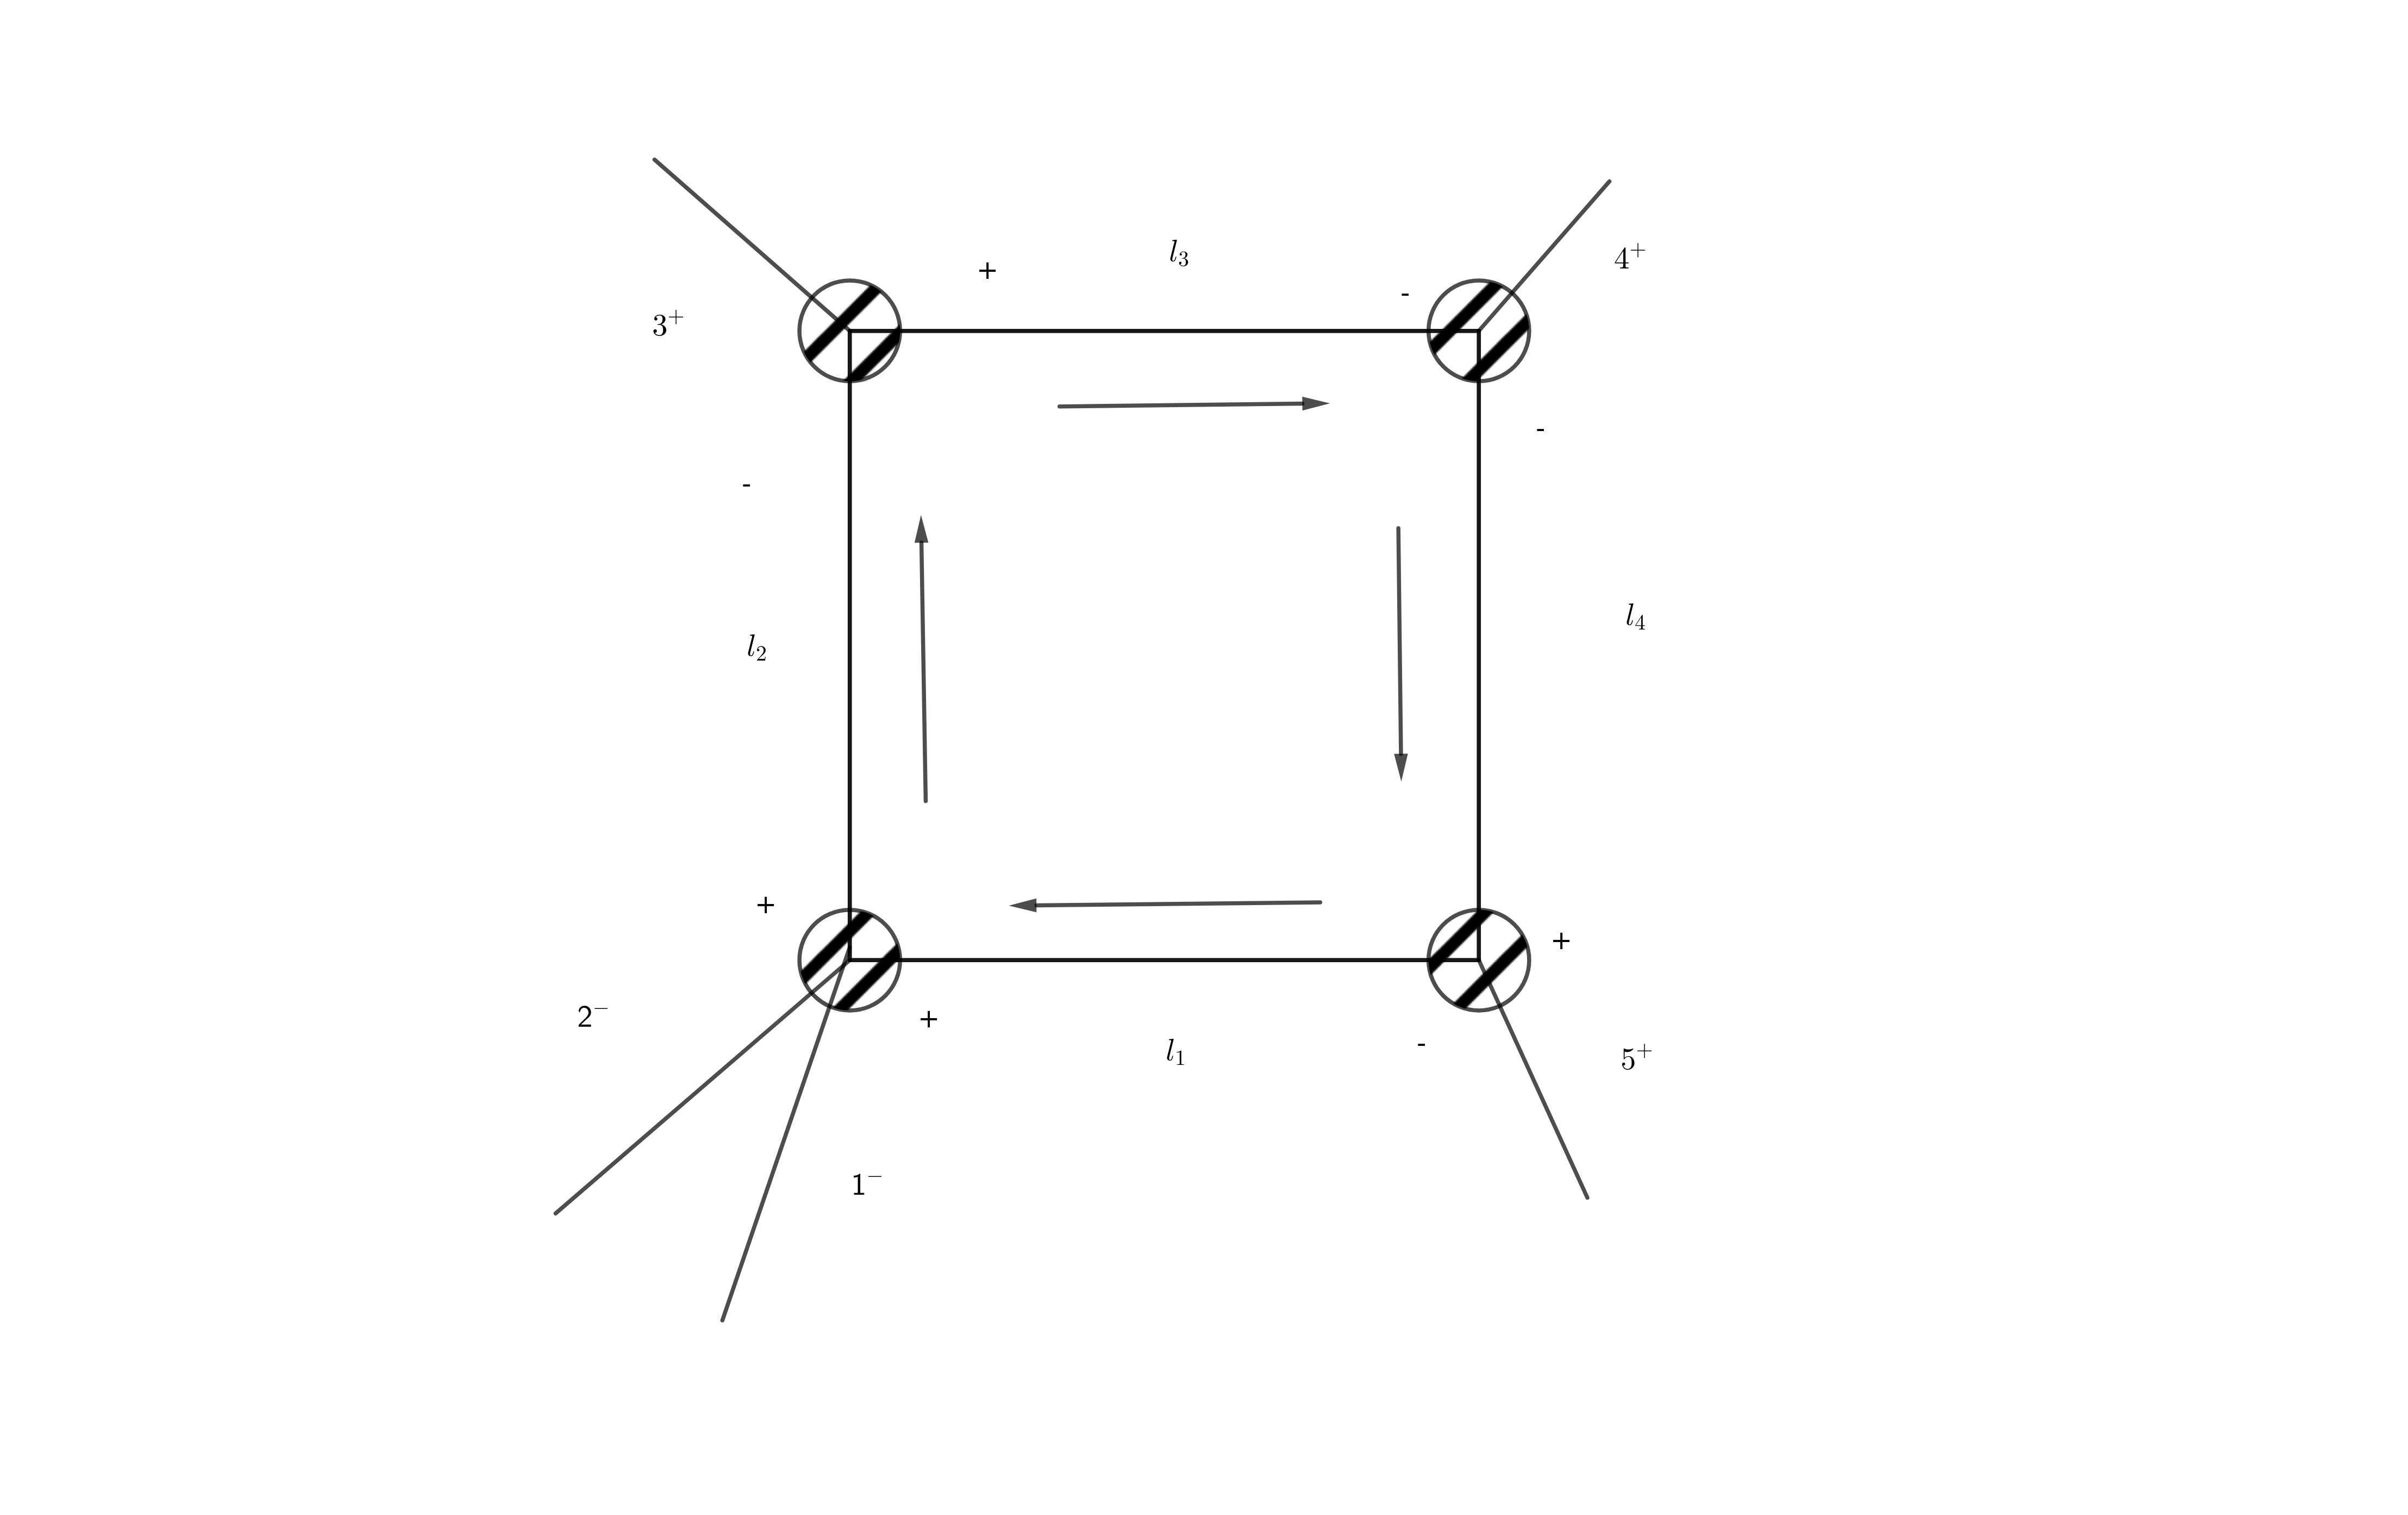
\includegraphics[width=\linewidth]{A5-1}
    \caption{A5-1}
  \label{A5-1}
\end{figure}
Let us now compute the box coefficients.
%
\paragraph{\ref{A5-1}}
The on-shell conditions allow us to set
\begin{equation*}
|l_1\rangle = \alpha |5\rangle \quad
|l_2\rangle = \delta |3\rangle \quad
|l_3\rangle = \gamma |l_3\rangle\quad
|l_3] = \eta|4]\quad
|l_4\rangle = \beta 4]
\end{equation*}
Hence, the coefficient
\begin{equation*}
\begin{split}
c_1 = &
\frac{1}{2}\frac{\langle 2 1 \rangle^4}{\langle 1 2 \rangle \langle 2 l_2\rangle \langle l_2 l_1 \rangle\langle l_1 1 \rangle}
\frac{[3l_3]^3}{[l_3 l_2][l_2 l_3]}
\frac{\langle l_3 l_4 \rangle^{3}}{\langle l_4 4 \rangle \langle 4 l_3\rangle}
\frac{[l_4 5 ]^3}{[5l_1][l_1 l_4]}
\\
= & 
\frac{1}{2}\frac{\langle 2 1 \rangle^3}{\langle 2 l_2 \rangle\langle l_2 l_1 \rangle\langle l_1 1\rangle}
\frac{[34]^2\langle 4 l_4\rangle}{[l_3 l_2][l_2 3]\langle 4 l_3\rangle}
\frac{[l_4 5]^2}{[5l_1 ][l_1 l_4]}
[3 l_3]\langle l_3 l_4 \rangle [l_4 l_5]
\\
= &
\frac{1}{2}\frac{\langle 21 \rangle^3 [34]^2 \langle 45 \rangle [45]}{\langle 32 \rangle \langle 5 | \slashed{K}_{12}|3]}
\end{split}
\end{equation*}
%
\color{gray}
We can use one of the on-shell conditions to get rid of the $\gamma\eta$ term
\begin{equation*}
-2l_3\cdot K_{123} = K_{123}^2 \Leftrightarrow \gamma\eta\langle 3 | \slashed{K}_{123}|4] = \gamma\eta\langle 3 | \slashed{K}_{12}|4] = K_{123}^2
\end{equation*}
Hence 
\begin{equation*}
c_1 = \frac{1}{2 K_{123}^2}\frac{\langle 2 1 \rangle^3 [34]\langle 45 \rangle\langle 3 | \slashed{K}_{12}|4]}{\langle 23 \rangle\langle 34 \rangle \langle 5 |\slashed{K}_{12}|3]}
\end{equation*}
\color{black}
%
\begin{figure}[h!]
  \centering
    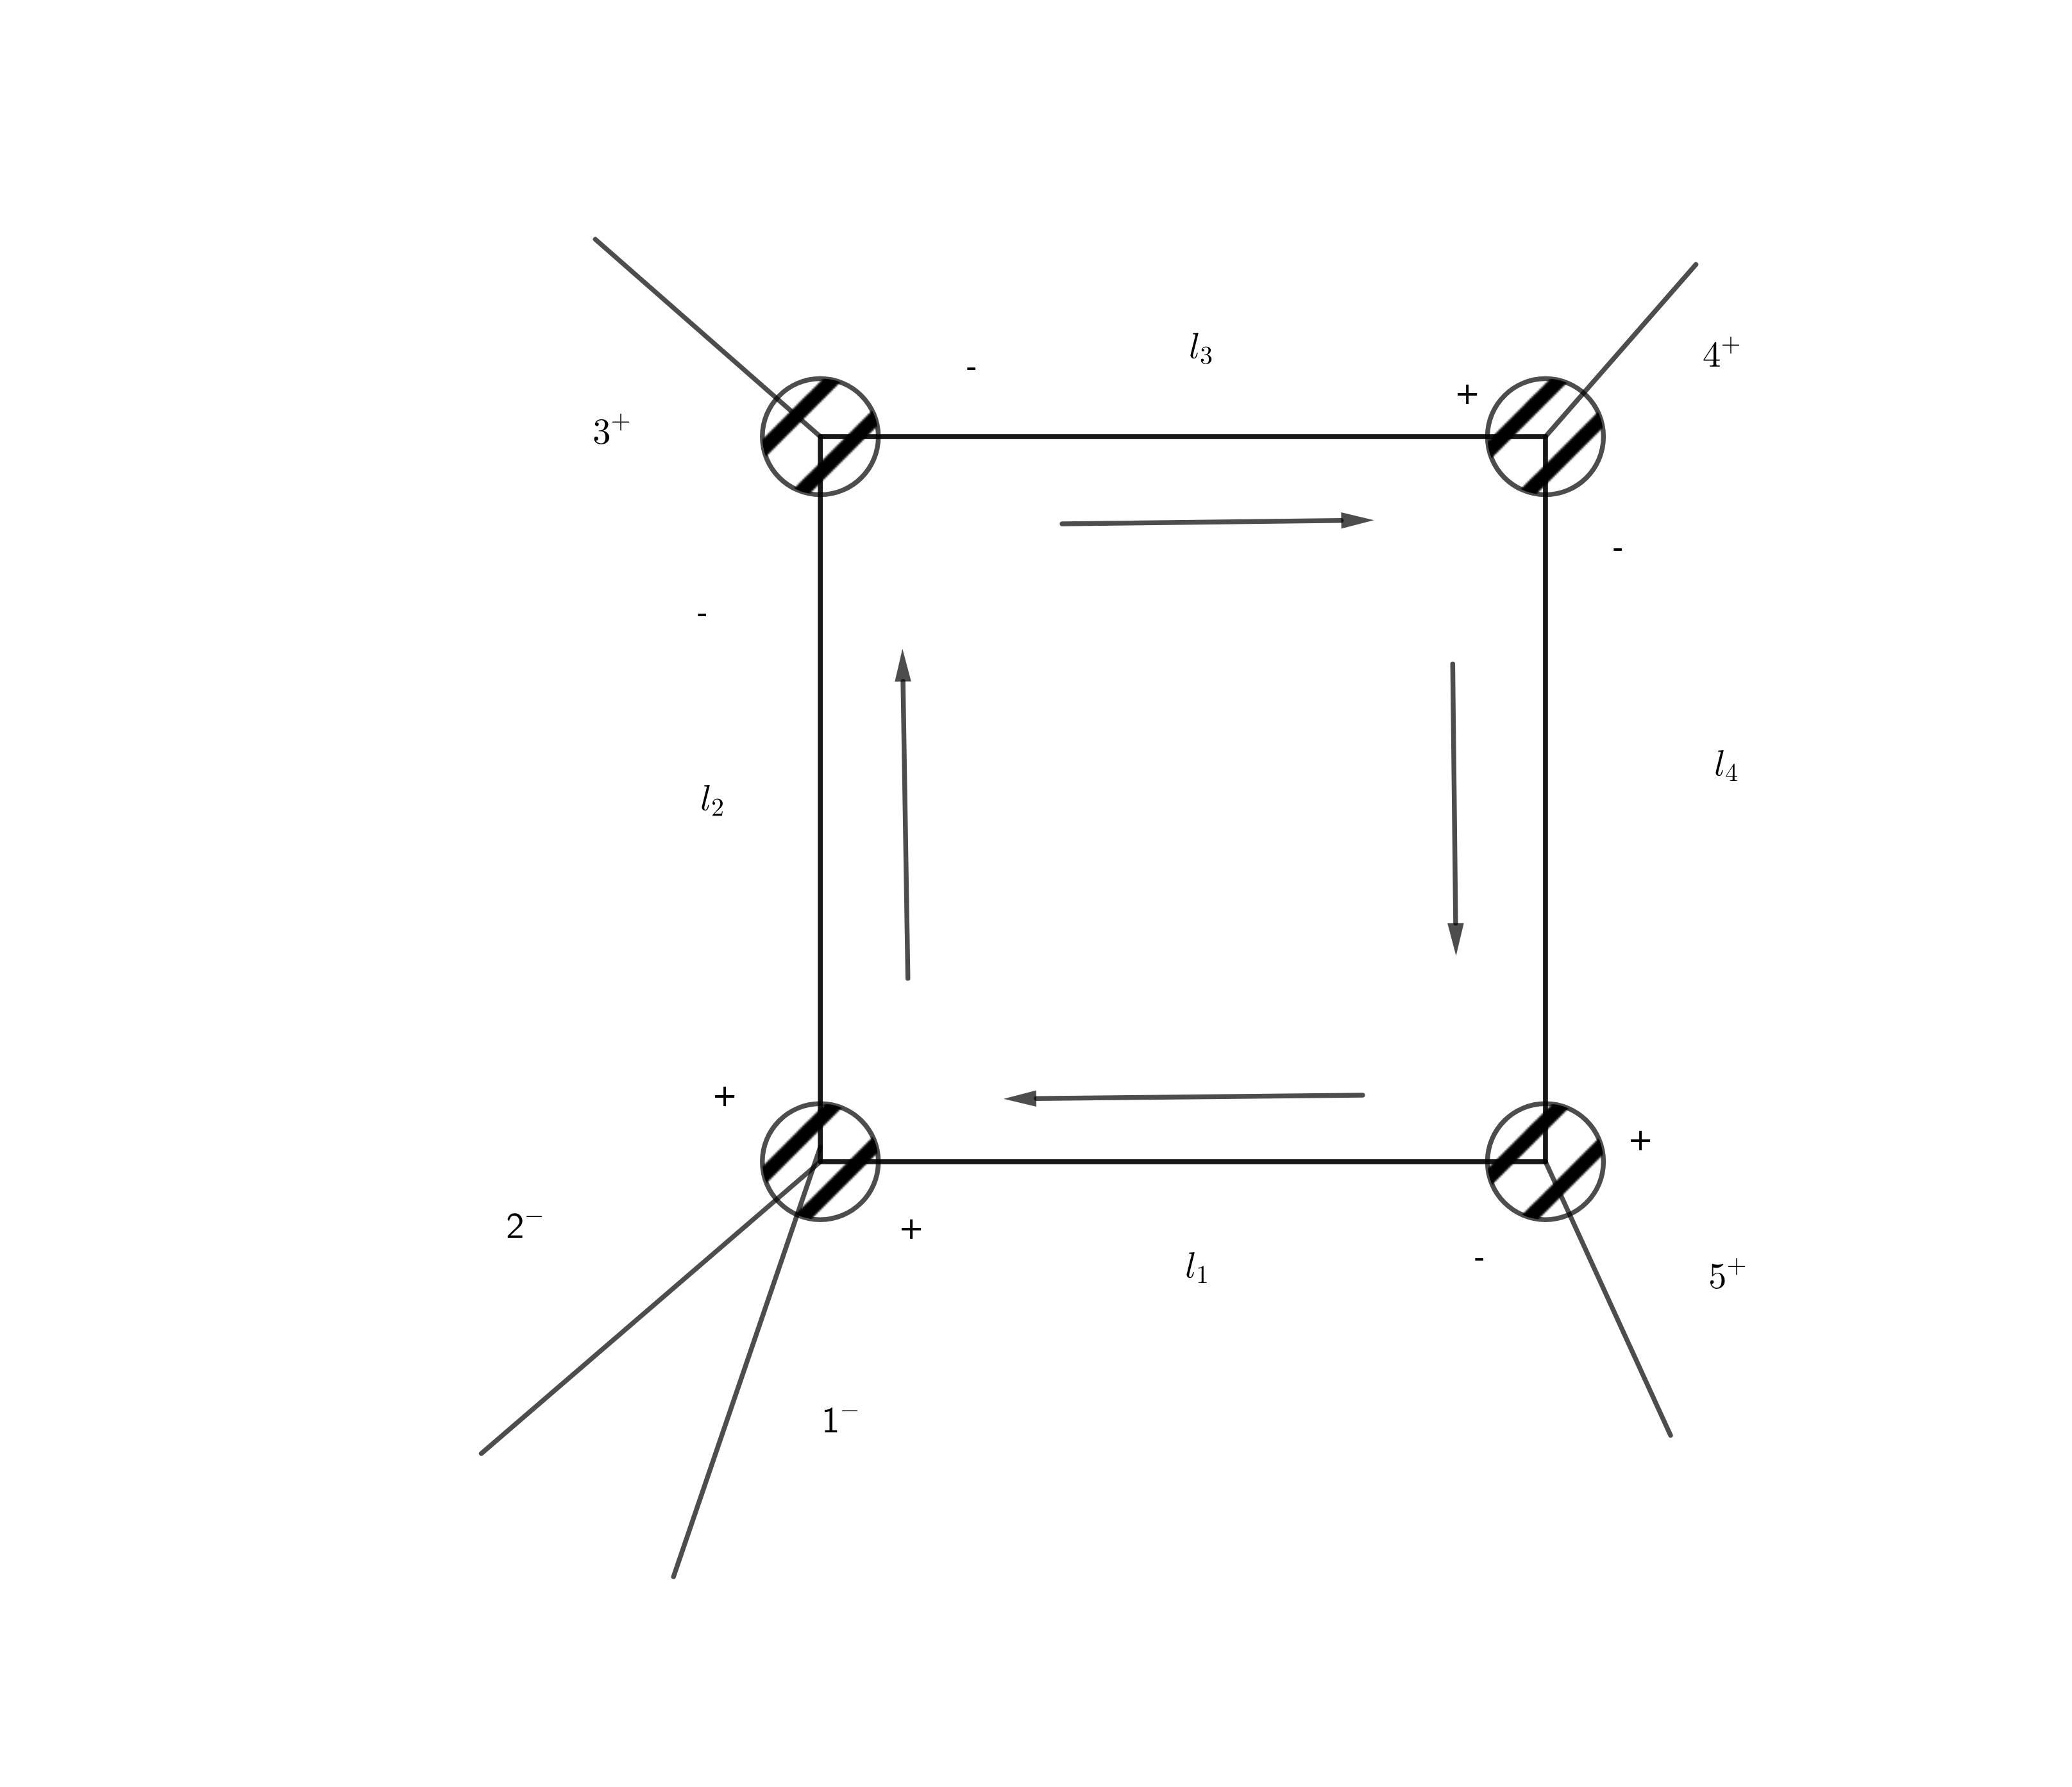
\includegraphics[width=\linewidth]{A5-2}
    \caption{A5-2}
  \label{A5-2}
\end{figure}
\paragraph{\ref{A5-2}}
%
\begin{equation*}
\begin{split}
c_2  = & \frac{1}{2}\frac{\langle 21 \rangle^4}{\langle 21 \rangle\langle 1 l_1 \rangle\langle l_1 l_2 \rangle\langle l_2 2 \rangle}
\frac{\langle l_2 l_3\rangle^3}{\langle 3 l_3 \rangle \langle l_3 l_2 \rangle}
\frac{[l_3 4]^3}{[4l_4][l_4 l_3]}
\frac{[5 l_4]^3}{[l_4 l_1][l_1 5]}
\\
= &
-\frac{1}{2}\frac{\langle 21 \rangle^3}{\langle 1 l_1 \rangle\langle l_1 l_2 \rangle\langle l_2 2 \rangle}
\frac{\langle l_2 3 \rangle^2[34]^3[5l_4]^3}{[l_4 3]\langle 3 4 \rangle [4 l_4][l_4 l_1][l_1 5]}
\\
= & 
\frac{1}{2}
\frac{\langle 21 \rangle^3 \langle l_2 3 \rangle^2 [34]^3 [5l_4]^2}{\langle 1 l_4 \rangle [l_4|\slashed{K}_{12}|l_2\rangle\langle l_2 2 \rangle [l_4 3]\langle 34 \rangle [4l_4]}
\end{split}
\end{equation*}
Due to the on-shell kinematic relations, we can write
\begin{equation*}
|l_3] = \alpha 3] \quad
|l_3\rangle = \beta |4\rangle \quad
|l_4\rangle = c|4\rangle \quad
|l_2] = f |3]
\end{equation*}
We re-express the remaining undetermined terms in using the on-shell conditions
\begin{equation*}
\langle l_3|\slashed{K}_{123}|l_3\rangle = K_{123}^2 \quad\Rightarrow
\alpha\beta \langle 4 | \slashed{K}_{123}|3] = K_{123}^2
\quad\Rightarrow
[4l_4]\langle l_4 1 \rangle = \alpha\beta [43]\langle 41 \rangle
=\frac{K_{123}^2}{\langle 4 |\slashed{K}_{123}|3]}[43]\langle 4 1 \rangle
\end{equation*}
Supposing
\begin{equation*}
|l_4] = a|3] + b|4] \quad
|l_2\rangle = d|3\rangle + e|4\rangle
\end{equation*}
we then have
\begin{equation*}
\begin{split}
&
(l_4 + K_{34})^2 = (l_4 + K_{1234})^2 = 0
\quad\Rightarrow
bc = \frac{K_{34}^2}{[4|\slashed{K}_3}|4\rangle
,\quad
ac = \frac{1}{[3|\slashed{K}_{12}|4\rangle}\Big(K_{1234}^2 - \frac{K_{34}^2 [4|\slashed{K}_{123}|4\rangle}{[4|\slashed{K}_3|4\rangle}\Big)
\\
&
(l_2 + K_{34} )^2 = (l_2 + K_{12})^2= 0 \quad\Rightarrow
df = \frac{K_{34}^2}{[3|\slashed{K}_4|3\rangle}
,\quad
de = \frac{1}{[3 | \slashed{K}_{12}|4\rangle}\Big(K_{12}^2 - \frac{[3|\slashed{K}_{12}|3\rangle K_{34}^2}{[3|\slashed{K}_4|3\rangle}\Big)
\end{split}
\end{equation*}
Since we have the same degree in loop spinors in the numerator and in the denominator, the exact values of $c$ and $f$ are not important.
%
\begin{figure}
  \centering
    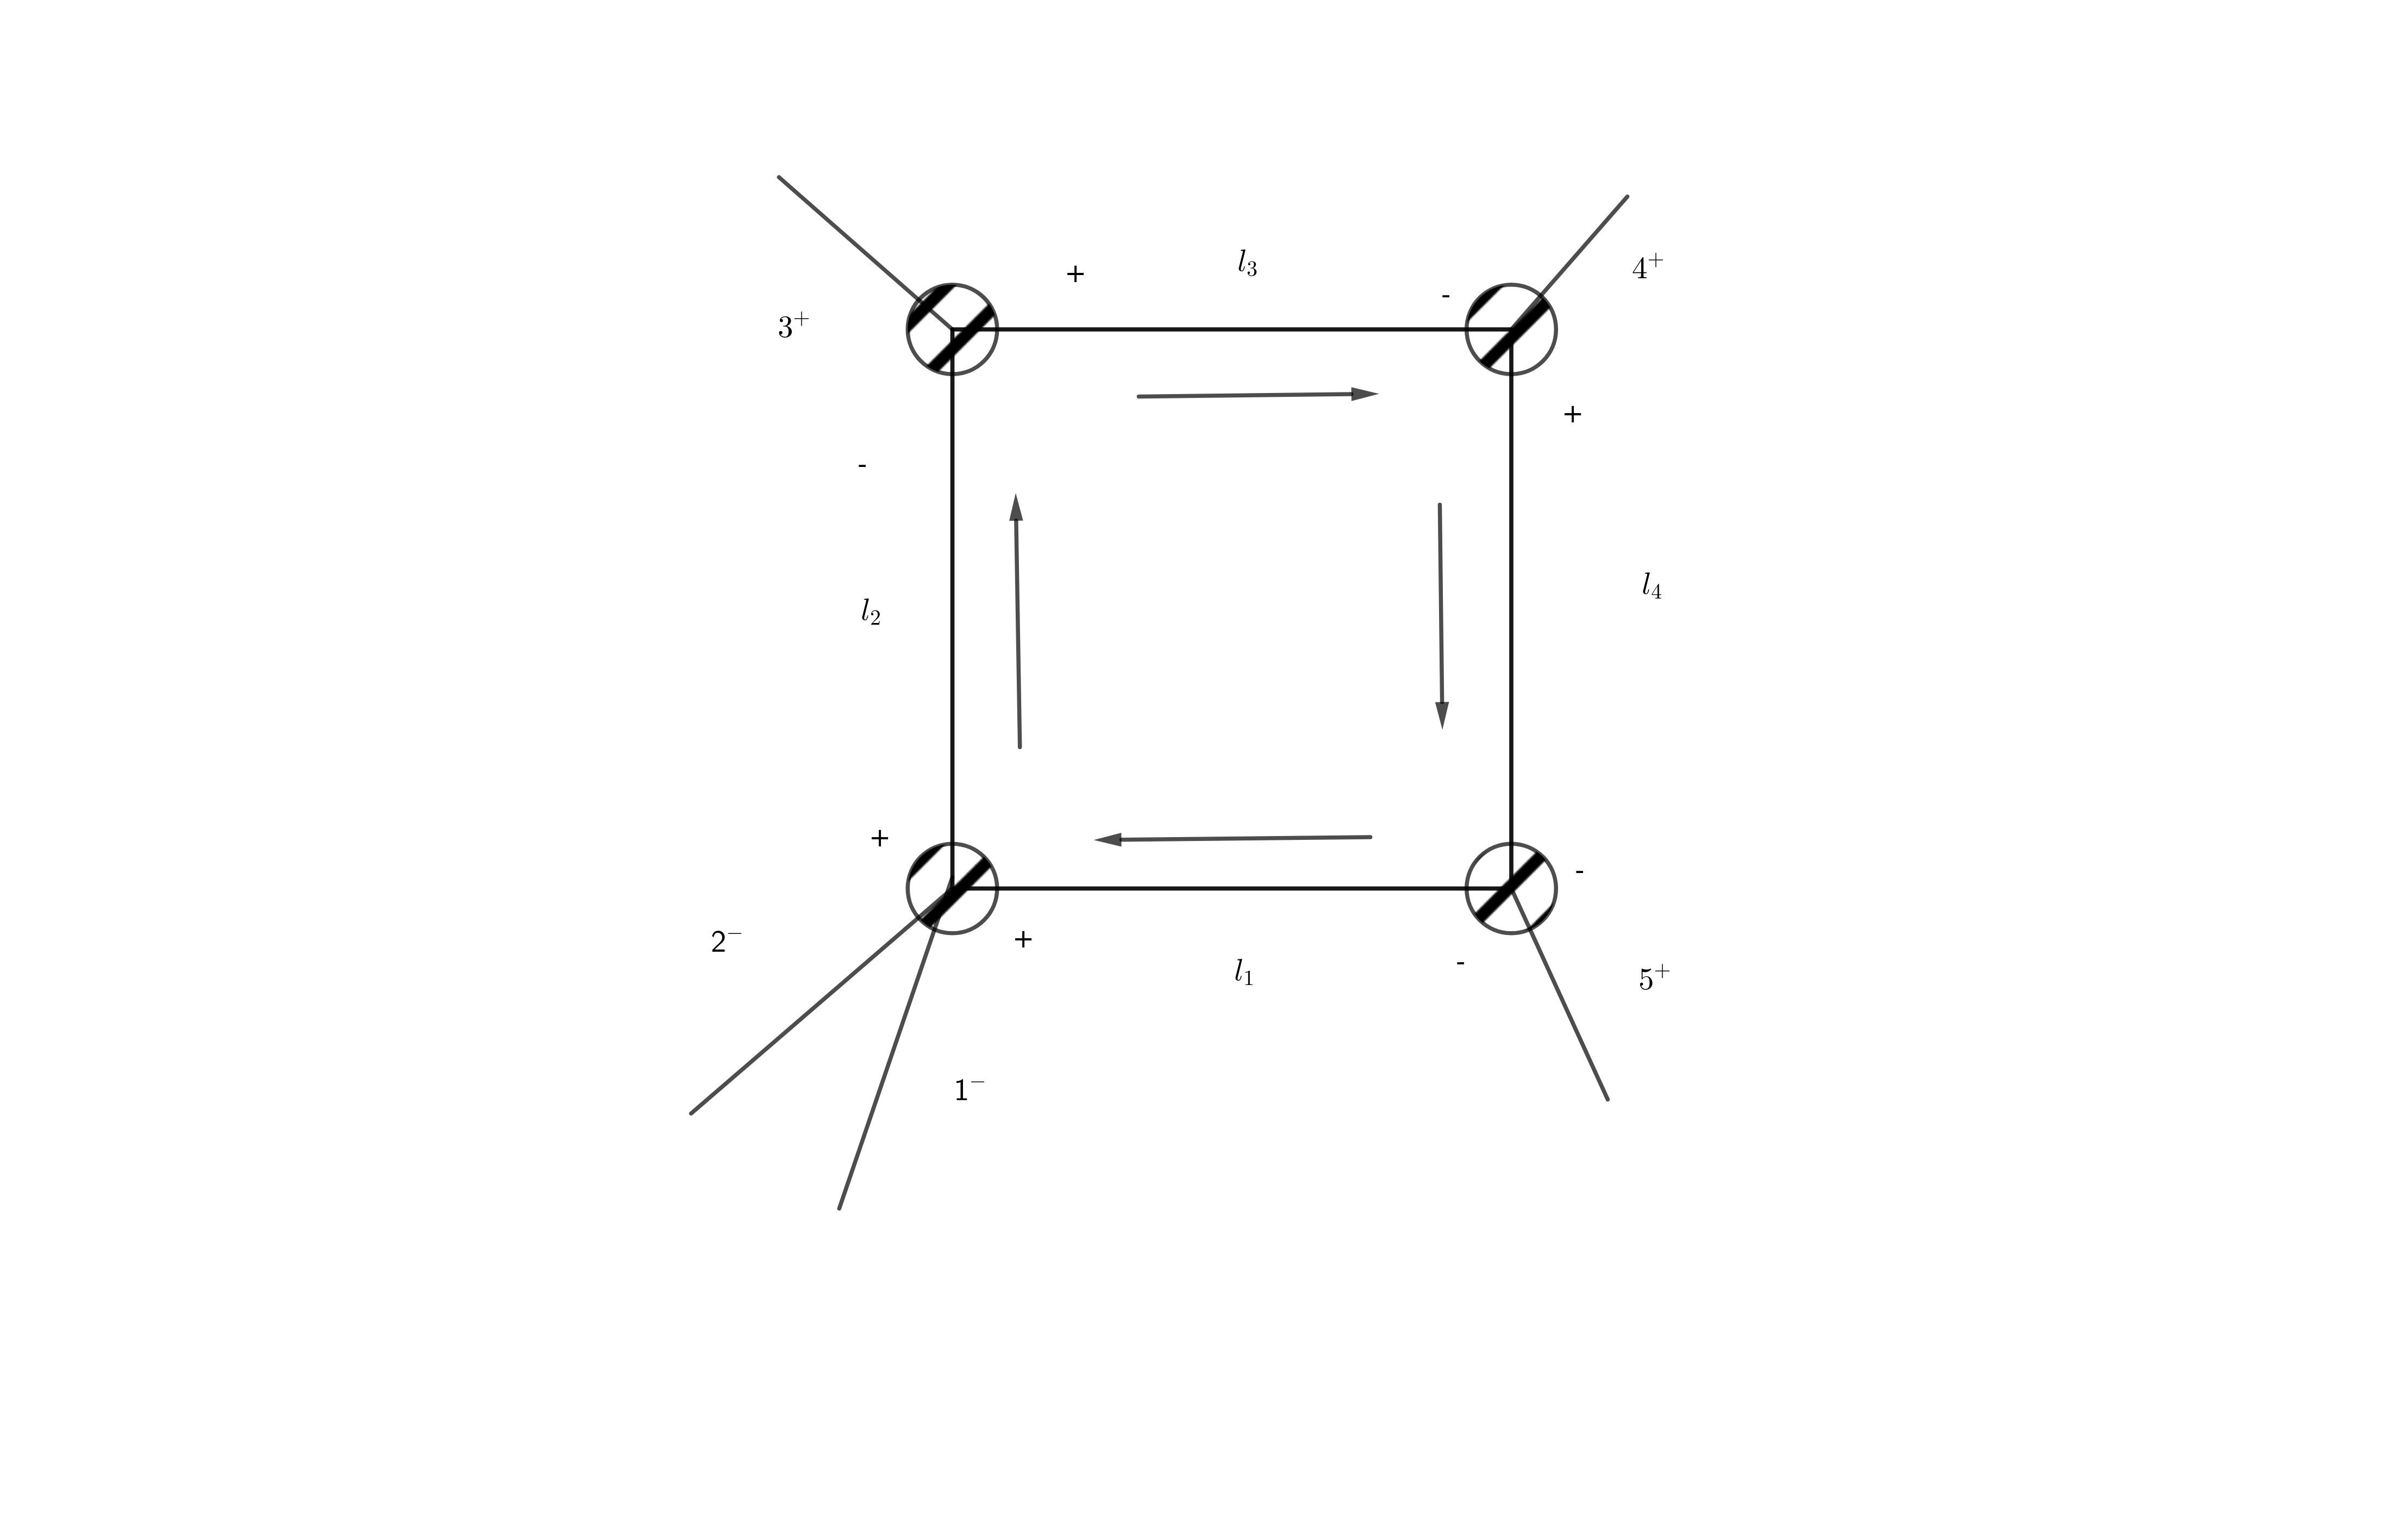
\includegraphics[width=\linewidth]{A5-3}
    \caption{A5-3}
  \label{A5-3}
\end{figure}
\paragraph{\ref{A5-3}}
\begin{equation*}
\begin{split}
c_3 = &
\frac{1}{2}
\frac{\langle 12 \rangle^4}{\langle 12 \rangle\langle 2l_2 \rangle\langle l_2 l_1 \rangle\langle l_1 1 \rangle}
\frac{[3l_3]^3}{[l_3 l_2][l_2 3]}
\frac{[4 l_3]^3}{[l_4 l_3][l_3 l_4]}
\frac{\langle l_4 l_1 \rangle^3}{\langle l_4 5\rangle\langle 5 l_1 \rangle}
\\
= &
\frac{1}{2}\frac{\langle 12 \rangle^3 [3|\slashed{K}_{12}|l_1\rangle^2}{\langle 23 \rangle [ 3 l_3]\langle l_1 1\rangle}\frac{[4l_3]}{\langle 45\rangle\langle 5l_1\rangle}
\end{split}
\end{equation*}
Set
\begin{equation*}
|l_1] = \alpha|5] ,\quad
|l_3\rangle = \beta|4\rangle, \quad
|l_1\rangle = a |4\rangle + b|5\rangle ,\quad
|l_3] = c|4] + d|5] 
\end{equation*}
Then
\begin{equation*}
\begin{split}
& (l_1 + K_{45})^2 = (l_1 - K_{12})^2 = 0 \quad\Rightarrow
\alpha b = \frac{-K_{45}^2}{[5|\slashed{K}_4|5\rangle} ,\quad
\alpha a = \frac{1}{[5|\slashed{K}_{12}|4\rangle}\Big(K_{12}^2 + \frac{K_{45}^2[5|\slashed{K}_4|5\rangle}{[5|\slashed{K}_{12}|5\rangle}\Big)
\\
& (l_3 -K_{45})^2 = (l_3 + K_3)^2 = 0 \quad\Rightarrow
\beta c =\frac{K_{45}^2}{[4|\slashed{K}_5|4\rangle} ,\quad
\beta d = \frac{1}{[5|\slashed{K}_3|4\rangle}\Big( -K_3^2 - \frac{K_{45}^2[4|\slashed{K}_3|4\rangle}{[4|\slashed{K}_5|4\rangle}\Big)
\end{split}
\end{equation*}
%
%
\begin{figure}
  \centering
    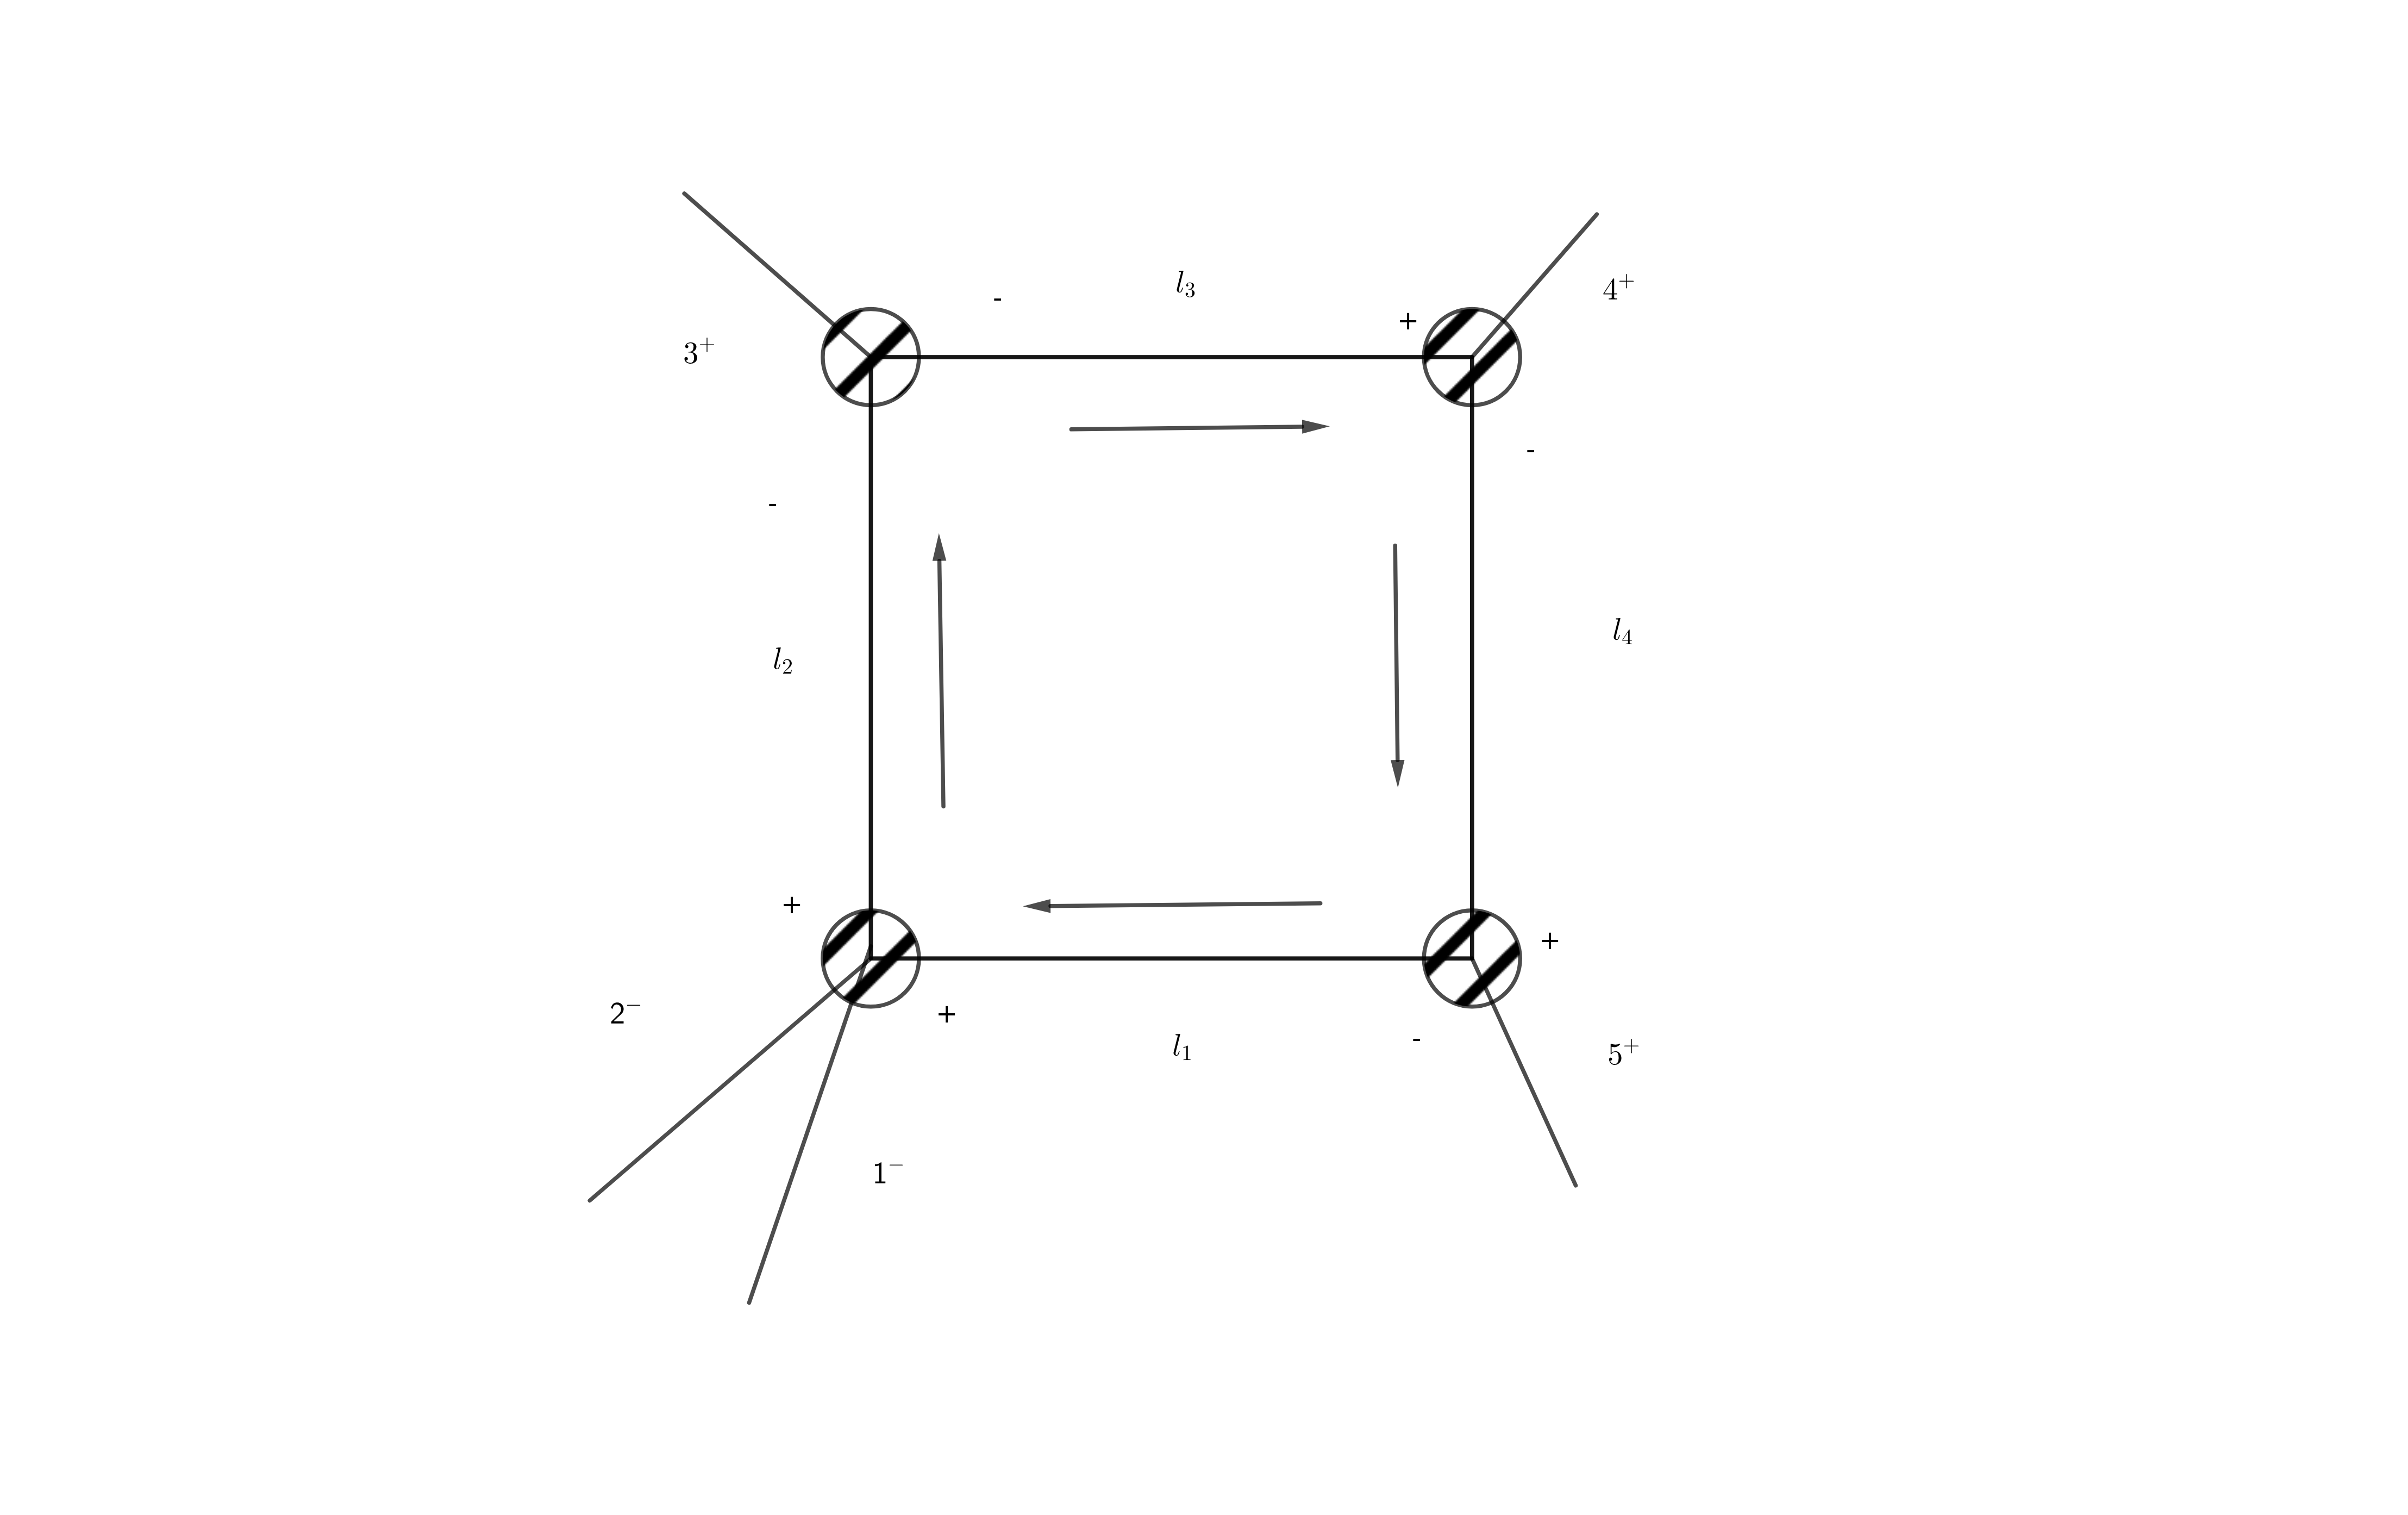
\includegraphics[width=\linewidth]{A5-4}
    \caption{A5-4}
  \label{A5-4}
\end{figure}
\paragraph{\ref{A5-4}}
\begin{equation*}
\begin{split}
c_4 = & \frac{1}{2}\frac{\langle 12 \rangle^4}{\langle 12 \rangle\langle 2l_2 \rangle\langle l_2 l_1 \rangle\langle l_1 1 \rangle}
\frac{\langle l_2 l_3 \rangle^3}{\langle l_2 3 \rangle \langle 3 l_3 \rangle}
\frac{[l_3 4 ]^3}{[l_4 l_3][4 l_4]}
\frac{[l_4 5]^3}{[5l_1][l_1 l_4]}
\\
= &
\frac{1}{2}\frac{\langle 12 \rangle^3}{\langle 2l_2\rangle\langle l_2 l_4 \rangle\langle 51 \rangle}
\frac{\langle l_2 3 \rangle^2 [34]^3 [l_4 5]}{\langle 3 l_3 \rangle [l_4 l_3][4 l_4]}
\\
= &
\frac{\langle 12 \rangle^3\langle l_2 3\rangle^2[34]^3[l_4 5]}{\langle 2 l_2 \rangle\langle l_2 l_4 \rangle\langle 51 \rangle\langle 34 \rangle [l_4 4]^2}
\end{split}
\end{equation*}
Set
\begin{equation*}
|l_2] = \alpha|3] \quad
|l_4\rangle = \beta|4\rangle \quad
|l_4] = a|3] + b|4] \quad
|l_2\rangle = c|3\rangle + d|4\rangle
\end{equation*}
We solve the coefficients with the on-shell conditions
\begin{equation*}
\begin{split}
& (l_4 + K_{34})^2 = (l_4 +K_{1234})^2 = 0 \quad\Rightarrow
b\beta = -\frac{K_{34}^2}{[4|\slashed{K}_3|4\rangle} ,\quad
a\beta = \frac{1}{[3|slashed{K}_{12}|4\rangle}\Big( -K_{1234}^2 + \frac{K_{34}^2 [4|\slashed{K}_{123}|4\rangle}{[4|\slashed{K}_3|4\rangle}\Big)
\\
&
(l_2 + K_{34})^2 = (l_2 + K_{1234})^2 = 0 \quad\Rightarrow
\alpha c = -\frac{K_{34}^2}{[3|\slashed{K}_4|3\rangle} ,\quad
\alpha d = \frac{1}{[3|\slashed{K}_{12}|4\rangle}\Big(-K_{1234}^2 + \frac{K_{34}^2 [3|\slashed{K}_{124}|3\rangle}{[3|\slashed{K}_4|3\rangle}\Big)
\end{split}
\end{equation*}